\section{Introduction}

The software/systems chosen for comparison in this project are two different NoSQL database system.  These systems will be deployed/run/operated in several different ways.  These include \emph{SaaS}\footnote{\textbf{SaaS :} Software as a service.} implementations, \emph{containerized} implementations, and \emph{native installations}.  The goal of the project is to understand the performance characteristics of each deployment method \emph{\textbf{and}} to quantify the costs of each deployment method.  These costs will be calculated based on the hourly cost to operate, the initial time \& costs required for setup, and the maintenance requirement of a deployment.  Additionally, performance of the systems and deployments will be measured using the time required to carry out various database operations, under a set of several different conditions, as well as the CPU, memory, and network loads imposed by the various deployments under the same set of conditions.




%---------------------------------------------------
%---------------------------------------------------



\section{Systems and Platforms}
We will be using two NoSQL database software packages.  The first software package is \textbf{DynamoDB} from Amazon Web Services (\emph{AWS}), while the second software package will be \textbf{Cassandra}, an open-source NoSQL database software package.  These software packages will be deployed using several different systems and platforms, as described below.



\subsection{Systems}

This project will run the software packages on three different systems (\emph{or types of systems}).  We have chosen systems which range from hosted \emph{SaaS} through various degrees of virtualization and then all the way to non-virtualized machines.  These systems are as follows

\begin{spacing}{1.40}
\begin{enumerate}[label=\Large{\textbf{\Alph*}):}]
	\item \textbf{\emph{SaaS}}
	\item \textbf{Running inside a \emph{Docker} container}
	\item \textbf{Running on a dedicated machine}
\end{enumerate}
\end{spacing}

These four systems will be deployed using several different platforms which we will describe in the next part of this section; however, before proceeding to that, we will give a through description of each system listed above.


\subsubsection{\underline{\emph{SaaS}} (code: \textbf{A}) }

In this system paradigm, a particular software package is developed and maintained with the intent of being used by a provider as selling \emph{Software as a Service}. As far as system configuration on our end (\emph{the system-administrator/developer}), paradigm only requires that we select a platform provider and collected the database data so that it can eventually be prepared for deployment.


\subsubsection{\underline{Running inside a \emph{Docker} container} (code: \textbf{B}) }

For the purposes for this paper and the ensuing project, we will only use \textbf{containers} which are created using and for use in \emph{Docker}.  This choice was made because of \emph{Docker}'s ubiquity, wide availability, and the ease of access to cloud services designed for and solely dedicated to the deployment of \emph{Docker} containers.  This implementation paradigm requires that a \emph{Docker} container be created after which, the software package in question be installed into the container so that it can be run on the operating system employed in the container (\emph{the OS\footnote{\textbf{OS: } Operating System} was chosen at the time of container creation}). Once the software has been installed, any information for and/or data required by it is either loaded into the container or, in the case of data \underline{\emph{only}}, the container is "pointed at" the location of the data required by the software.  Finally, we must note that, as far as this paper and project are concerned, the use of a \emph{Docker} container as a means of implementation does not imply the use of any particular platform for running the containers, or even a deployment of the \emph{Docker} software/system itself. 


\subsubsection{\underline{Running on a dedicated machine} (code: \textbf{C}) }

The third system paradigm involves acquiring and configuring a dedicated machine which can be either an actual, physical machine or a virtual machine.  In either case, the machine will have performance specifications and and run an OS appropriate for our planed use.  When setting up one of these machines, after configuration and setup of physical/virtual system, the selected OS will be installed and configured for use.  Once it has been verified that the OS has been properly installed and configured (\emph{i.e. running stably}) we will install the software selected for testing on that instance, along with any other software or system components required to run that software.  After configuring the installed software, the machine will be prepared and configured for use as a server running said software.  The final step of this paradigm is preparing the software and system combination for final deployment to the selected platform.



%---------------------------------------------------


\subsection{Platforms}

We have chosen four different platforms on which to deploy our systems.  The chosen platforms span the range of cloud service paradigms from \emph{SaaS} to \emph{PaaS}\footnote{\textbf{PaaS :} Platform as a service.} to \emph{IaaS}\footnote{\textbf{IaaS :} Infrastructure as a service.}.  We list the three platforms, along with two variations on one of the platforms, below

\begin{spacing}{1.40}
\begin{enumerate}[label=\Large{\textbf{\arabic*}):}]
	\item \textbf{(An) AWS Software Service (}\emph{SaaS}\textbf{)}
	%\item \textbf{AWS \emph{SaaS} system(s)}
	\item \textbf{Containers (}using \emph{Docker}\textbf{) running on}

	\begin{enumerate}[label=\Large{\textbf{\roman*}):}]
		\item \textbf{\emph{AWS's Container Service} (}\emph{PaaS}\textbf{)}
		\item \textbf{\emph{AWS EC2 VM with Docker run-time} (}hybrid \emph{Pass/IaaS}\textbf{)}
	\end{enumerate}
	\vspace{0.025in}
	
	\item \textbf{AWS EC2 VMs running the software in Linux (}\emph{IaaS}\textbf{)}
	\item \textbf{A dedicated, non-virtualized server (}\emph{server}\textbf{)}
\end{enumerate}
\end{spacing}


In the next section, we list which systems will run each software package, along with a explanation why each software-system pairing was chosen.  Additionally, we will describe which platforms will be used to deploy each system and why those deployment choices were made.  Before proceeding to that, and as with our list of system, we will describe each platform thoroughly.


\subsubsection{\underline{AWS Software Service} (code: \textbf{1})}

Our first platform we will use for the deployment of some systems is AWS's Software Service platform which provides various software packages which run as a service.  This means that Administrator do not have to configure and secure a server and OS on which to run the software, nor do they have to install and manage the running of the software on said server.  Instead, all a System Administrator must do is create an instance of the desired Software Service, with the configuration required for the application at hand.  Once the instance has been created, it is loaded with any information required and/or data to be used, after which it is immediately available for use by users and other clients. 


\subsubsection{\underline{Containers} (code: \textbf{2\_})}\footnote{In the code \textbf{2\_}, we use the "\_" after the 2 is a place-holder for an additional code-letter.  This is due to the fact that two different versions of and approaches to this platform (\emph{container deployment}) are going to be used.}

The next platform we have chosen involves the deployment of the previously described \emph{Docker} containers.  We will use two different platforms that implement the \emph{Docker} engine which is actually responsible for running the containers.  These "\emph{Docker} Platforms" are

\begin{quote}
\begin{itemize}
	\vspace{0.05in}
	\item $\bigl[$\normalsize{\emph{\underline{AWS's Container Service} (code:} \textbf{2i}\emph{)}}$\bigr]\text{\Large{\textbf{:}}}$ In this version of the second platform, we will deploy our containers by using AWS's Container Service.  When deploying to this platform, an Administrator first creates an appropriately configured instance of the Container Service.  Upon the successful creation and launch of the Container Service instance in question, the Administrator simply uploads the container being deployed to the instance and, if a data-source external to the container is required, uploads the required data to the location specified during the creation of the container.  Once the container has been uploaded to the instance (\emph{and any required data has been uploaded to the appropriate location}), the Administrator tests the instance to ensure it is functioning as expected.  In the last step, the Administrator configures the instance to properly connect with users and/or clients before finally granting them access to the deployed container. 
	\vspace{0.075in}
	\item $\bigl[$\normalsize{\emph{\underline{AWS EC2 VM with Docker run-time} (code:} \textbf{2ii}\emph{)}}$\bigr] \text{\Large{\textbf{:}}}$ The other version of the second deployment platform involves deploying our containers using a \emph{Docker} run-time/engine running in a Linux machine being hosted on AWS's EC2 Virtualization Platform.  To deploy via this platform, an Administrator begins by creating an EC2 VM instance with performance characteristics necessary for running the container inside the Linux version of \emph{Docker} run-time.  Once the EC2 VM instance has been created and successfully launched, the Administrator will install and configure an appropriate version of Linux, followed by installing the \emph{Docker} run-time and any required support software (\emph{such as software for accessing remotely stored data}).  After configuring the installation of the \emph{Docker} run-time (\emph{and any support software}), the Administrator will upload the container using \emph{Docker}.  

Additionally, if a data-source external to the container is employed, up to two additional steps are required and based on whether the data is local or remote to the VM instance.  In the case the data-source is local to the VM instance, the Administrator must also configure appropriate storage on the instance, including installing and configuring any necessary software, after which the required data is uploaded to the storage location.  Similarly, if the data-source is external to the VM instance, the Administrator must also install and configure the software required for accessing the remote location (\emph{NFS, SAN, Samba, EBS, etc}), followed by configuring the system to access the remote location and the data stored within.  Once these steps are complete, the Administrator will be able configure the container to run on the VM instance, as well as configure 

the OS to allow the container to properly run.  These configurations involve ensuring that the container has access to the necessary networks, addresses, and ports and that any local and/or remote resources are both appropriately mounted to the container (\emph{container configuration}) and accessible to the container (\emph{OS configuration}).  With these configurations complete, the Administrator is able to launch the container and begin testing it to ensure it functions as expected.  Once the container has been determined to be properly functioning, the Administrator completes any configuration of the EC2 Instance, the VM itself (\emph{OS}), and the container itself which might be necessary for proper user and/or client access of the container.  This final configuration is followed, finally, by allowing users and clients to access the container.
\end{itemize}
\end{quote}


\subsubsection{\underline{AWS EC2 VMs running the software in Linux} (code: \textbf{3})}

Our third deployment platform paradigm also relies on use of AWS's EC2 VM service; however, instead of installing using containers as in \textbf{\underline{2ii}}, this paradigm has the software to be tested natively and directly installed on a Linux OS being run on an AWS EC2 VM instance.  As with the previous paradigm involving an AWS EC2 VM the Administrator begins by creating an EC2 VM instance, launching it, and installing an appropriate version of the Linux operating system, with the only difference being the determination of necessary performance characteristics base on natively running the software, and any supporting software, in Linux.  Following the installation and configuration of the Linux OS, the Administrator will natively install and then configure the software to be tested, along with any other software required support software (\emph{i.e. remote data access}).  These installations are followed by creating and configuring any required local storage space on the instance, to include installing and configuring any software necessary for doing this.  In the case where remote storage be used instead of or in addition to local storage, the Administrator must also install and configure the software required for accessing the remote location, followed by configuring the system to access the remote location and the data stored within.  Once these data storage/access steps have been completed, the Administrator uploads the required data to the appropriate location or locations, after which they configure both the software being tested, so that it can locate these data-sources, and the OS, so the software can access both the data-sources and any required networks, services, or ports.  As before, this configuration step is followed first by testing to ensure the software is accessible and works as desired, and then by the final step, allowing users and clients to access the container.


\subsubsection{\underline{A dedicated, non-virtualized server} (code: \textbf{4})}

The last deployment platform we have chosen is a dedicated, non-virtualized server.  These servers will run Linux as their OS and will be dedicated to running and serving the software to be tested.









%%%%%%%
%\vspace{3in}
%$a \in \text{\large{\textbf{TaCo}}} \ni a \equiv \text{\large{\textbf{\emph{yummy}}}}$ \new
\newpage
%%%%%%%




%---------------------------------------------------
%---------------------------------------------------



\section{Deployment}

The deployment strategy will be described in two parts which can be briefly described as "\emph{what systems will be used to run and/or implement each software package}" and "\emph{which platforms will be used to deploy each of these systems}".  Specifically, the first part of the description for our deployment strategy details which systems will be used to run each software package (\emph{DynamoDB \underline{or} Cassandra}), along with how the each system will implement and run the software.  This will be complemented by the second part of the description, which will detail what platforms will be used for deploying each of the systems, along with why each platform was chosen to deploy are particular software/system combination.  




























































\newpage


\newpage










\subsection{Math Equations}
You may want to display math equations in three distinct styles:
inline, numbered or non-numbered display.  Each of
the three are discussed in the next sections.

\subsubsection{Inline (In-text) Equations}
A formula that appears in the running text is called an
inline or in-text formula.  It is produced by the
\textbf{math} environment, which can be
invoked with the usual \texttt{{\char'134}begin\,\ldots{\char'134}end}
construction or with the short form \texttt{\$\,\ldots\$}. You
can use any of the symbols and structures,
from $\alpha$ to $\omega$, available in
\LaTeX~\cite{Lamport:LaTeX}; this section will simply show a
few examples of in-text equations in context. Notice how
this equation:
\begin{math}
  \lim_{n\rightarrow \infty}x=0
\end{math},
set here in in-line math style, looks slightly different when
set in display style.  (See next section).

\subsubsection{Display Equations}
A numbered display equation---one set off by vertical space from the
text and centered horizontally---is produced by the \textbf{equation}
environment. An unnumbered display equation is produced by the
\textbf{displaymath} environment.

Again, in either environment, you can use any of the symbols
and structures available in \LaTeX\@; this section will just
give a couple of examples of display equations in context.
First, consider the equation, shown as an inline equation above:
\begin{equation}
  \lim_{n\rightarrow \infty}x=0
\end{equation}
Notice how it is formatted somewhat differently in
the \textbf{displaymath}
environment.  Now, we'll enter an unnumbered equation:
\begin{displaymath}
  \sum_{i=0}^{\infty} x + 1
\end{displaymath}
and follow it with another numbered equation:
\begin{equation}
  \sum_{i=0}^{\infty}x_i=\int_{0}^{\pi+2} f
\end{equation}
just to demonstrate \LaTeX's able handling of numbering.

\subsection{Citations}
Citations to articles~\cite{bowman:reasoning,
clark:pct, braams:babel, herlihy:methodology},
conference proceedings~\cite{clark:pct} or maybe
books \cite{Lamport:LaTeX, salas:calculus} listed
in the Bibliography section of your
article will occur throughout the text of your article.
You should use BibTeX to automatically produce this bibliography;
you simply need to insert one of several citation commands with
a key of the item cited in the proper location in
the \texttt{.tex} file~\cite{Lamport:LaTeX}.
The key is a short reference you invent to uniquely
identify each work; in this sample document, the key is
the first author's surname and a
word from the title.  This identifying key is included
with each item in the \texttt{.bib} file for your article.

The details of the construction of the \texttt{.bib} file
are beyond the scope of this sample document, but more
information can be found in the \textit{Author's Guide},
and exhaustive details in the \textit{\LaTeX\ User's
Guide} by Lamport~\shortcite{Lamport:LaTeX}.


This article shows only the plainest form
of the citation command, using \texttt{{\char'134}cite}.

\subsection{Tables}
Because tables cannot be split across pages, the best
placement for them is typically the top of the page
nearest their initial cite.  To
ensure this proper ``floating'' placement of tables, use the
environment \textbf{table} to enclose the table's contents and
the table caption.  The contents of the table itself must go
in the \textbf{tabular} environment, to
be aligned properly in rows and columns, with the desired
horizontal and vertical rules.  Again, detailed instructions
on \textbf{tabular} material
are found in the \textit{\LaTeX\ User's Guide}.

Immediately following this sentence is the point at which
Table~\ref{tab:freq} is included in the input file; compare the
placement of the table here with the table in the printed
output of this document.

\begin{table}
  \caption{Frequency of Special Characters}
  \label{tab:freq}
  \begin{tabular}{ccl}
    \toprule
    Non-English or Math&Frequency&Comments\\
    \midrule
    \O & 1 in 1,000& For Swedish names\\
    $\pi$ & 1 in 5& Common in math\\
    \$ & 4 in 5 & Used in business\\
    $\Psi^2_1$ & 1 in 40,000& Unexplained usage\\
  \bottomrule
\end{tabular}
\end{table}

To set a wider table, which takes up the whole width of the page's
live area, use the environment \textbf{table*} to enclose the table's
contents and the table caption.  As with a single-column table, this
wide table will ``float'' to a location deemed more desirable.
Immediately following this sentence is the point at which
Table~\ref{tab:commands} is included in the input file; again, it is
instructive to compare the placement of the table here with the table
in the printed output of this document.


\begin{table*}
  \caption{Some Typical Commands}
  \label{tab:commands}
  \begin{tabular}{ccl}
    \toprule
    Command &A Number & Comments\\
    \midrule
    \texttt{{\char'134}author} & 100& Author \\
    \texttt{{\char'134}table}& 300 & For tables\\
    \texttt{{\char'134}table*}& 400& For wider tables\\
    \bottomrule
  \end{tabular}
\end{table*}
% end the environment with {table*}, NOTE not {table}!

It is strongly recommended to use the package booktabs~\cite{Fear05}
and follow its main principles of typography with respect to tables:
\begin{enumerate}
\item Never, ever use vertical rules.
\item Never use double rules.
\end{enumerate}
It is also a good idea not to overuse horizontal rules.


\subsection{Figures}

Like tables, figures cannot be split across pages; the best placement
for them is typically the top or the bottom of the page nearest their
initial cite.  To ensure this proper ``floating'' placement of
figures, use the environment \textbf{figure} to enclose the figure and
its caption.

This sample document contains examples of \texttt{.eps} files to be
displayable with \LaTeX.  If you work with pdf\LaTeX, use files in the
\texttt{.pdf} format.  Note that most modern \TeX\ systems will convert
\texttt{.eps} to \texttt{.pdf} for you on the fly.  More details on
each of these are found in the \textit{Author's Guide}.

\begin{figure}
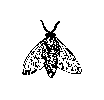
\includegraphics{fly}
\caption{A sample black and white graphic.}
\end{figure}

\begin{figure}
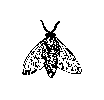
\includegraphics[height=1in, width=1in]{fly}
\caption{A sample black and white graphic
that has been resized with the \texttt{includegraphics} command.}
\end{figure}


As was the case with tables, you may want a figure that spans two
columns.  To do this, and still to ensure proper ``floating''
placement of tables, use the environment \textbf{figure*} to enclose
the figure and its caption.  And don't forget to end the environment
with \textbf{figure*}, not \textbf{figure}!

\begin{figure*}
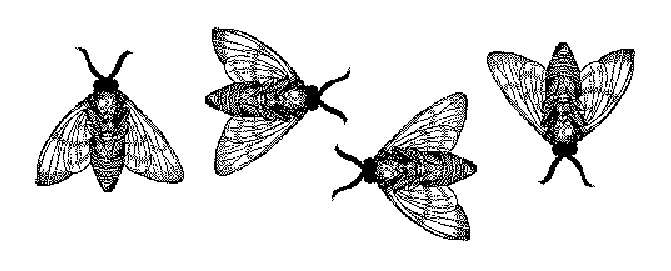
\includegraphics{flies}
\caption{A sample black and white graphic
that needs to span two columns of text.}
\end{figure*}


\begin{figure}

\includegraphics[height=1in, width=1in]{rosette}
\caption{A sample black and white graphic that has
been resized with the \texttt{includegraphics} command.}
\end{figure}

\subsection{Theorem-like Constructs}

Other common constructs that may occur in your article are the forms
for logical constructs like theorems, axioms, corollaries and proofs.
ACM uses two types of these constructs:  theorem-like and
definition-like.

Here is a theorem:
\begin{theorem}
  Let $f$ be continuous on $[a,b]$.  If $G$ is
  an antiderivative for $f$ on $[a,b]$, then
  \begin{displaymath}
    \int^b_af(t)\,dt = G(b) - G(a).
  \end{displaymath}
\end{theorem}

Here is a definition:
\begin{definition}
  If $z$ is irrational, then by $e^z$ we mean the
  unique number that has
  logarithm $z$:
  \begin{displaymath}
    \log e^z = z.
  \end{displaymath}
\end{definition}

The pre-defined theorem-like constructs are \textbf{theorem},
\textbf{conjecture}, \textbf{proposition}, \textbf{lemma} and
\textbf{corollary}.  The pre-defined de\-fi\-ni\-ti\-on-like constructs are
\textbf{example} and \textbf{definition}.  You can add your own
constructs using the \textsl{amsthm} interface~\cite{Amsthm15}.  The
styles used in the \verb|\theoremstyle| command are \textbf{acmplain}
and \textbf{acmdefinition}.

Another construct is \textbf{proof}, for example,

\begin{proof}
  Suppose on the contrary there exists a real number $L$ such that
  \begin{displaymath}
    \lim_{x\rightarrow\infty} \frac{f(x)}{g(x)} = L.
  \end{displaymath}
  Then
  \begin{displaymath}
    l=\lim_{x\rightarrow c} f(x)
    = \lim_{x\rightarrow c}
    \left[ g{x} \cdot \frac{f(x)}{g(x)} \right ]
    = \lim_{x\rightarrow c} g(x) \cdot \lim_{x\rightarrow c}
    \frac{f(x)}{g(x)} = 0\cdot L = 0,
  \end{displaymath}
  which contradicts our assumption that $l\neq 0$.
\end{proof}

\section{Conclusions}
This paragraph will end the body of this sample document.
Remember that you might still have Acknowledgments or
Appendices; brief samples of these
follow.  There is still the Bibliography to deal with; and
we will make a disclaimer about that here: with the exception
of the reference to the \LaTeX\ book, the citations in
this paper are to articles which have nothing to
do with the present subject and are used as
examples only.
%\end{document}  % This is where a 'short' article might terminate



\appendix
%Appendix A
\section{Headings in Appendices}
The rules about hierarchical headings discussed above for
the body of the article are different in the appendices.
In the \textbf{appendix} environment, the command
\textbf{section} is used to
indicate the start of each Appendix, with alphabetic order
designation (i.e., the first is A, the second B, etc.) and
a title (if you include one).  So, if you need
hierarchical structure
\textit{within} an Appendix, start with \textbf{subsection} as the
highest level. Here is an outline of the body of this
document in Appendix-appropriate form:
\subsection{Introduction}
\subsection{The Body of the Paper}
\subsubsection{Type Changes and  Special Characters}
\subsubsection{Math Equations}
\paragraph{Inline (In-text) Equations}
\paragraph{Display Equations}
\subsubsection{Citations}
\subsubsection{Tables}
\subsubsection{Figures}
\subsubsection{Theorem-like Constructs}
\subsubsection*{A Caveat for the \TeX\ Expert}
\subsection{Conclusions}
\subsection{References}
Generated by bibtex from your \texttt{.bib} file.  Run latex,
then bibtex, then latex twice (to resolve references)
to create the \texttt{.bbl} file.  Insert that \texttt{.bbl}
file into the \texttt{.tex} source file and comment out
the command \texttt{{\char'134}thebibliography}.
% This next section command marks the start of
% Appendix B, and does not continue the present hierarchy
\section{More Help for the Hardy}

Of course, reading the source code is always useful.  The file
\path{acmart.pdf} contains both the user guide and the commented
code.

\begin{acks}
  The authors would like to thank Dr. Yuhua Li for providing the
  matlab code of  the \textit{BEPS} method. 

  The authors would also like to thank the anonymous referees for
  their valuable comments and helpful suggestions. The work is
  supported by the \grantsponsor{GS501100001809}{National Natural
    Science Foundation of
    China}{http://dx.doi.org/10.13039/501100001809} under Grant
  No.:~\grantnum{GS501100001809}{61273304}
  and~\grantnum[http://www.nnsf.cn/youngscientsts]{GS501100001809}{Young
    Scientsts' Support Program}.

\end{acks}
